\documentclass{beamer}

\usepackage{amsmath}
\usepackage[italian]{babel}
\usepackage{bookmark}
\usepackage{booktabs}
\usepackage{boxedminipage}
\usepackage{svg}

\setlength{\fboxrule}{0pt}
\usetheme{Rochester}

\title{Studio e approfondimento del coefficiente Silhouette per la
valutazione interna di risultati di clustering non-supervisionato}
\author{Federico Salvioni 845029}
\date{\today}

\begin{document}

    \begin{frame}
        \titlepage
    \end{frame}

    \section{Clustering}

        \begin{frame}
            \frametitle{Clustering}

            \vfill

            \begin{block}{Cluster}
                \emph{``A number of similar things that occur together''}
            \end{block}

            \vfill

            \begin{block}{Cluster analysis}
                \emph{``A statistical classification technique for discovering
                      whether the individuals of a population fall into different groups
                      by making quantitative comparisons of multiple characteristics''}
            \end{block}
        \end{frame}

        \begin{frame}
            \frametitle{Quanti e quali sono i cluster?}

            \begin{itemize}
                \item
                Gli algoritmi di clustering non supervisionato non sono in
                grado di determinare se il loro operato rispecchi la struttura
                di cluster, perché non vi è alcuna "ground truth";
                \item
                Utilizzare parametri errati induce un raggruppamento non
                rappresentativo del dataset, senza che l'algoritmo lo
                consideri un errore;
                \item
                Sono state proposte diverse metriche che sono in grado di
                stimare la qualità dell'operato di un algoritmo di clustering
                non supervisionato.
            \end{itemize}
        \end{frame}

    \section{Silhouette}

        \begin{frame}
            \frametitle{Introduzione di Silhouette}

            La metrica Silhouette si propone di rispondere alle seguenti domande:
        
            \begin{itemize}
                \item
                Il clustering è di buona qualità?
                \item
                Quali elementi sono stati ben classificati?
                \item
                Quali elementi sono inclassificabili?
                \item
                Il numero di cluster scelto è rappresentativo del dataset?
            \end{itemize}

            \vfill
            Questo è possibile a partire da una nozione di \textbf{distanza}.
        \end{frame}

        \begin{frame}
            \frametitle{Formula per la Silhouette}

            \centering
            \begin{boxedminipage}{0.49\textwidth}
                \begin{block}{$a(i)$}
                    \begin{equation*}
                        a(i) = \frac{1}{|A| - 1} \sum_{j \in \{A - \{i\}\}} d(i, j)
                    \end{equation*}
                \end{block}
            \end{boxedminipage}
            \begin{boxedminipage}{0.49\textwidth}
                \begin{block}{$b(i)$}
                    \begin{equation*}
                        b(i) = min_{C \neq A} \frac{1}{|C|} \sum_{j \in C} d(i, j)
                    \end{equation*}
                \end{block}
            \end{boxedminipage}

            \vfill

            \begin{block}{$s(i)$}
                \begin{equation*}
                    s(i) = \frac{b(i) - a(i)}{max\{a(i), b(i)\}}
                \end{equation*}
            \end{block}
        \end{frame}

        \begin{frame}
            \frametitle{Silhouette width}

            \centering
            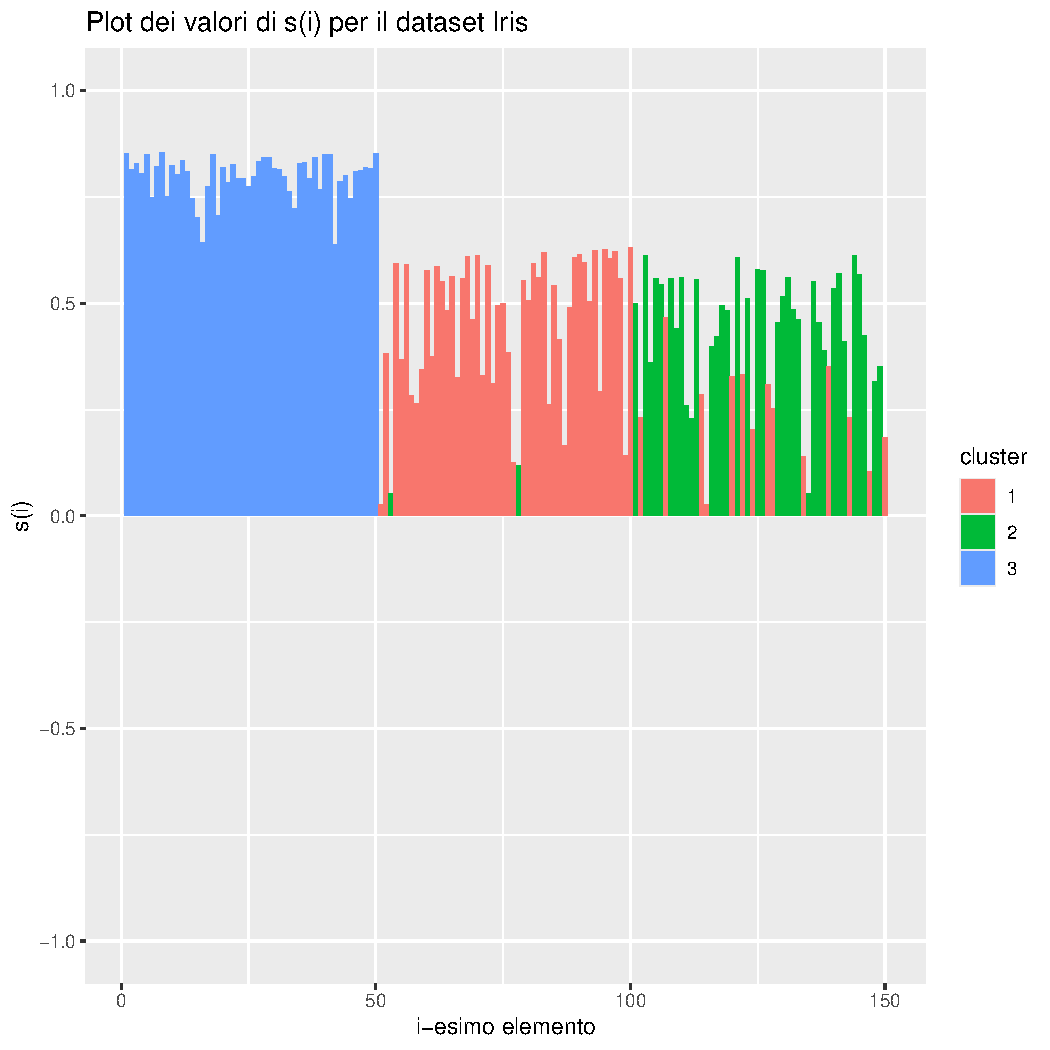
\includegraphics[width = 0.65\textwidth]{doc/si.pdf}
        \end{frame}

    \section{Clustering}

        \begin{frame}
            \frametitle{Algoritmi di clustering}

            \centering
            \begin{boxedminipage}{0.49\textwidth}
                \begin{figure}
                \includesvg[width = 0.9\textwidth]{images/K-Means-Example.svg}
                \caption{K-Means}
                \end{figure}
            \end{boxedminipage}
            \begin{boxedminipage}{0.49\textwidth}
                \begin{figure}
                \includesvg[width = 0.9\textwidth]{images/DBSCAN-density-data.svg}
                \caption{DBSCAN}
                \end{figure}
            \end{boxedminipage}
        \end{frame}

    \section{Test}

        \begin{frame}
            \frametitle{Matrice binaria}

            \centering
            \begin{boxedminipage}{0.49\textwidth}
                \begin{figure}
                    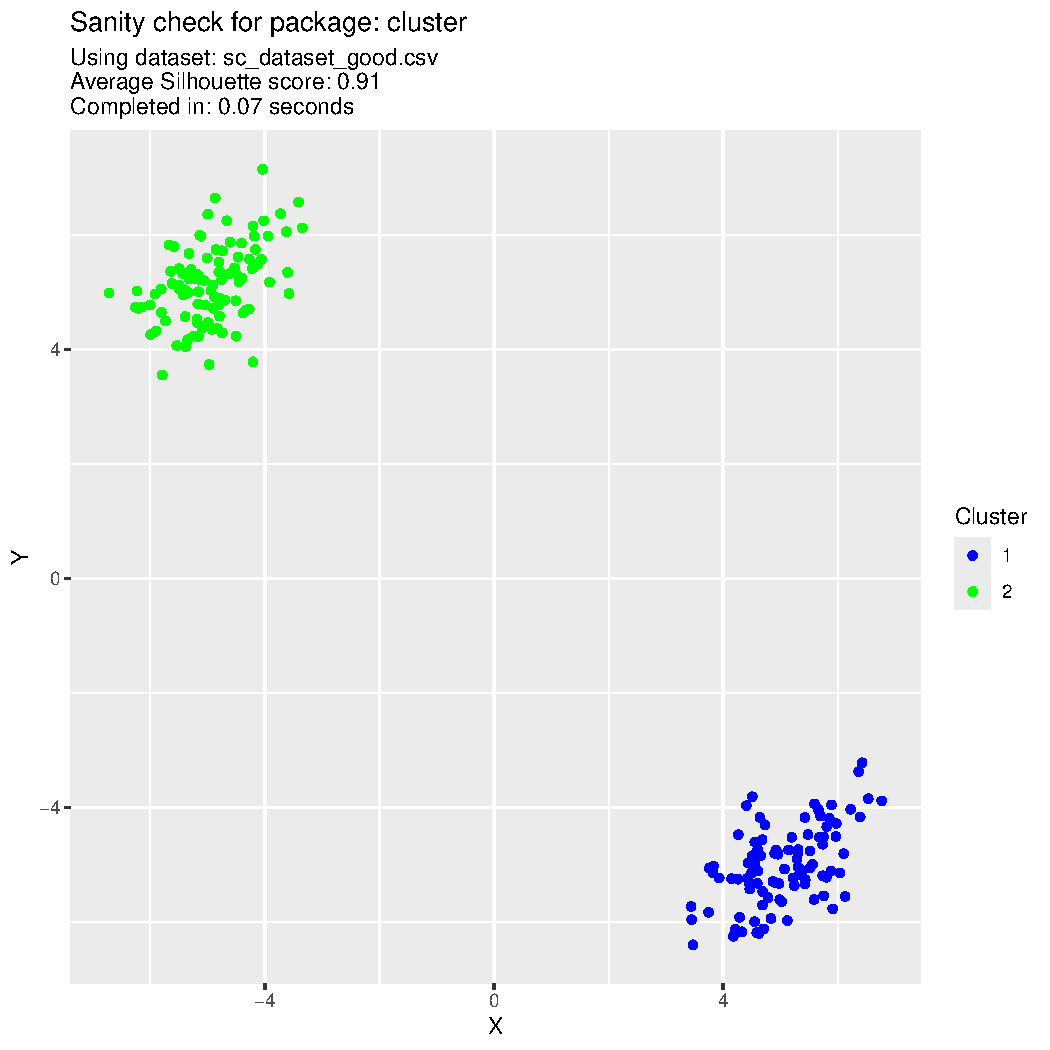
\includegraphics[width = \textwidth, page = 1]{results/results_CLUSTER.pdf}
                    \caption{Sanity check (favorevole)}
                \end{figure}
            \end{boxedminipage}
            \begin{boxedminipage}{0.49\textwidth}
                \begin{figure}
                    \includegraphics[width = \textwidth, page = 2]{results/results_CLUSTER.pdf}
                    \caption{Sanity check (sfavorevole)}
                \end{figure}
            \end{boxedminipage}
        \end{frame}

        \begin{frame}
            \frametitle{Sanity check}

            \centering
            \begin{boxedminipage}{0.49\textwidth}
                \begin{figure}
                    \includegraphics[width = \textwidth, page = 3]{results/results_CLUSTER.pdf}
                    \caption{Matrice binaria}
                \end{figure}
            \end{boxedminipage}
            \begin{boxedminipage}{0.49\textwidth}
                \begin{figure}
                    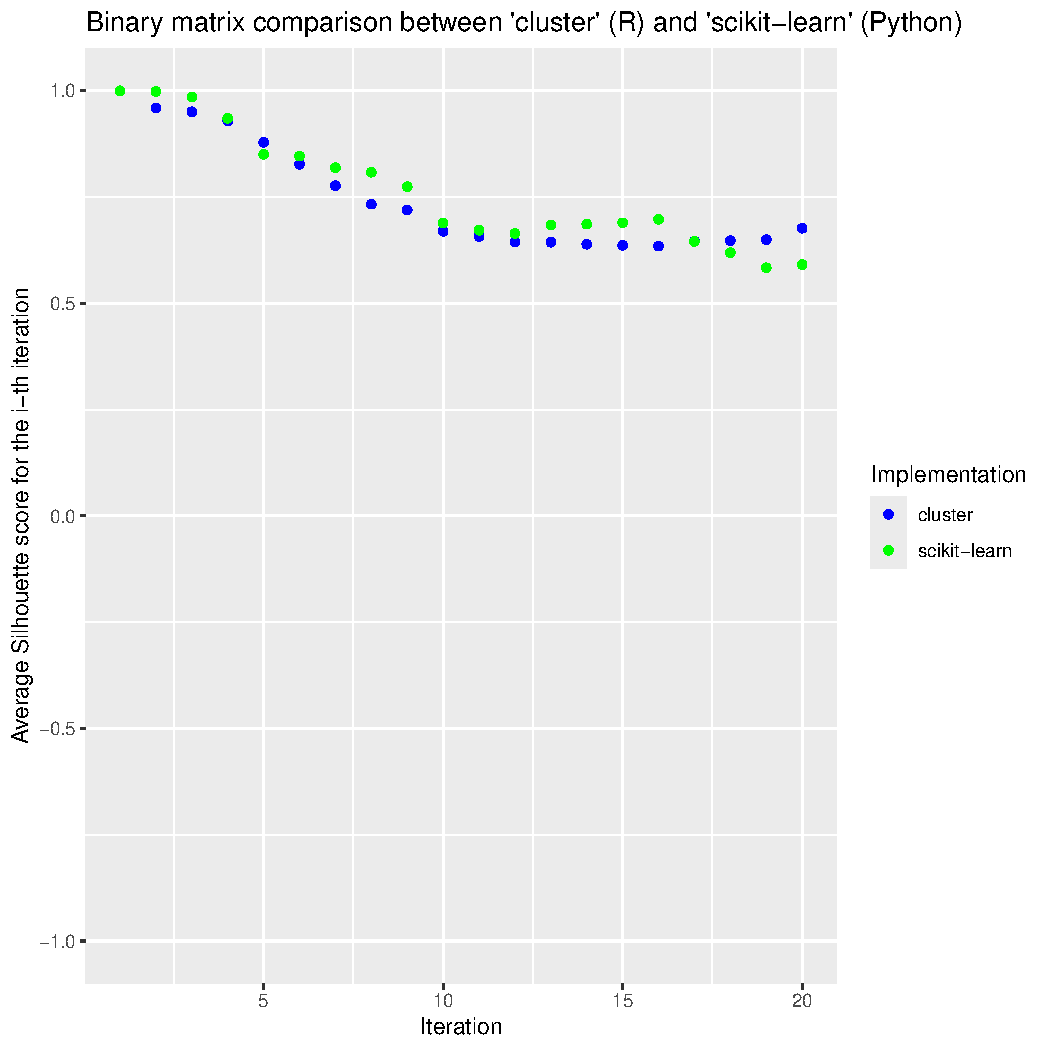
\includegraphics[width = \textwidth, page = 1]{results/Final_comparison.pdf}
                    \caption{Comparazione R/Python}
                \end{figure}
            \end{boxedminipage}
        \end{frame}

    \section{EHR}

        \begin{frame}
            \frametitle{Clustering su dataset reali}

	    \centering
            \begin{boxedminipage}{0.49\textwidth}
                \begin{figure}
                    \includegraphics[width = \textwidth, page = 7]{results/results_Neuroblastoma.csv.pdf}
                    \caption{Elbow plot}
                \end{figure}
            \end{boxedminipage}
            \begin{boxedminipage}{0.49\textwidth}
                \begin{figure}
                    \includegraphics[width = \textwidth, page = 8]{results/results_Neuroblastoma.csv.pdf}
                    \caption{Clustering}
                \end{figure}
            \end{boxedminipage}
        \end{frame}

	\begin{frame}
            \frametitle{Clustering su dataset reali}

	    \centering
            \begin{boxedminipage}{0.49\textwidth}
                \begin{figure}
                    \includegraphics[width = \textwidth, page = 9]{results/results_Neuroblastoma.csv.pdf}
                    \caption{Ranking (1)}
                \end{figure}
            \end{boxedminipage}
            \begin{boxedminipage}{0.49\textwidth}
                \begin{figure}
                    \includegraphics[width = \textwidth, page = 10]{results/results_Neuroblastoma.csv.pdf}
                    \caption{Ranking (2)}
                \end{figure}
            \end{boxedminipage}
        \end{frame}

    \section{Conclusioni}

        \begin{frame}
            \frametitle{Sviluppi futuri}

            Possibili estensioni:

            \begin{itemize}
                \item Usare dataset che non siano EHR;
                \item Sostituire i valori ignoti con valori concreti, anziché scartare gli elementi manchevoli;
                \item Ridurre il numero di dimensioni (\textbf{principal component analysis}).
            \end{itemize}
        \end{frame}

    \section{Fine}

        \begin{frame}
            \frametitle{Fine}
            \centering
            \Huge{Domande?}

            
\includegraphics{images/Chill.png}
        \end{frame}

\end{document}
